\documentclass[border=4pt]{standalone}
\usepackage{tikz}
\usetikzlibrary{arrows.meta,positioning,calc,fit,backgrounds,patterns,shapes.geometric}
\usepackage{amsmath,amssymb}
\usepackage{mathptmx}
\definecolor{lost}{HTML}{C2362D}
\definecolor{kept}{HTML}{17875A}
\definecolor{evid}{HTML}{3056D3}
\definecolor{ink}{HTML}{1D1D1F}
\definecolor{muted}{HTML}{6E6E73}
\tikzset{
  box/.style={draw=ink!70, rounded corners=2pt, align=center, fill=white, inner sep=4pt, font=\footnotesize},
  arr/.style={-{Stealth[length=2mm]}, draw=ink!70, line width=0.6pt},
  grp/.style={draw=muted!60, dashed, rounded corners=4pt, inner sep=7pt},
  lossbox/.style={draw=lost!80, fill=lost!6, text=lost!85!black, rounded corners=2pt, align=left, font=\footnotesize, inner sep=4pt},
  fixbox/.style={draw=kept!80, fill=kept!7, text=kept!65!black, rounded corners=2pt, align=left, font=\footnotesize, inner sep=4pt},
  dec/.style={diamond, aspect=2.2, draw=ink!70, fill=evid!6, align=center, font=\footnotesize, inner sep=1.5pt},
  lbl/.style={font=\footnotesize\bfseries, text=ink},
}

\begin{document}
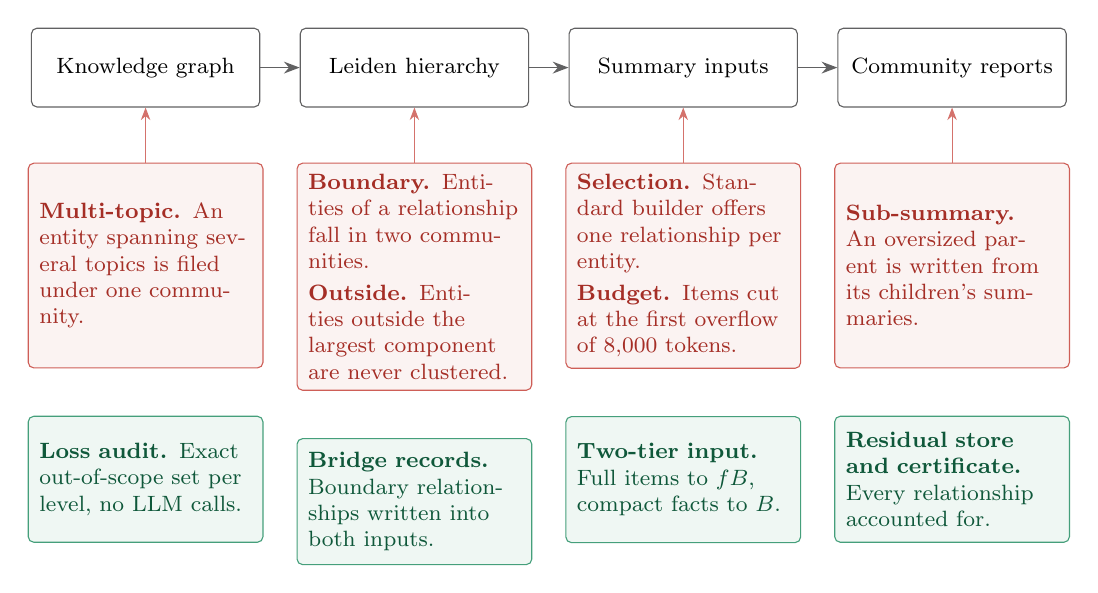
\begin{tikzpicture}[node distance=0.5cm]
\node[box, minimum width=2.9cm, minimum height=1.0cm] (a) {Knowledge graph};
\node[box, minimum width=2.9cm, minimum height=1.0cm, right=of a] (b) {Leiden hierarchy};
\node[box, minimum width=2.9cm, minimum height=1.0cm, right=of b] (c) {Summary inputs};
\node[box, minimum width=2.9cm, minimum height=1.0cm, right=of c] (d) {Community reports};
\foreach \x/\y in {a/b,b/c,c/d} \draw[arr] (\x) -- (\y);
\node[lossbox, text width=2.7cm, below=0.7cm of b, minimum height=2.6cm] (l1) {\textbf{Boundary.} Entities of a relationship fall in two communities.\\[2pt]\textbf{Outside.} Entities outside the largest component are never clustered.};
\node[lossbox, text width=2.7cm, below=0.7cm of c, minimum height=2.6cm] (l2) {\textbf{Selection.} Standard builder offers one relationship per entity.\\[2pt]\textbf{Budget.} Items cut at the first overflow of 8,000 tokens.};
\node[lossbox, text width=2.7cm, below=0.7cm of d, minimum height=2.6cm] (l3) {\textbf{Sub-summary.} An oversized parent is written from its children's summaries.};
\node[lossbox, text width=2.7cm, below=0.7cm of a, minimum height=2.6cm] (l0) {\textbf{Multi-topic.} An entity spanning several topics is filed under one community.};
\foreach \l/\n in {l0/a,l1/b,l2/c,l3/d} \draw[-{Stealth[length=1.6mm]}, draw=lost!70] (\l.north) -- (\n.south);
\node[fixbox, text width=2.7cm, below=0.6cm of l0, minimum height=1.6cm] (f0) {\textbf{Loss audit.} Exact out-of-scope set per level, no LLM calls.};
\node[fixbox, text width=2.7cm, below=0.6cm of l1, minimum height=1.6cm] (f1) {\textbf{Bridge records.} Boundary relationships written into both inputs.};
\node[fixbox, text width=2.7cm, below=0.6cm of l2, minimum height=1.6cm] (f2) {\textbf{Two-tier input.} Full items to $fB$, compact facts to $B$.};
\node[fixbox, text width=2.7cm, below=0.6cm of l3, minimum height=1.6cm] (f3) {\textbf{Residual store and certificate.} Every relationship accounted for.};
\end{tikzpicture}
\end{document}
